\section{Methods}

The methodology presented determines a Pareto Front of the \gls{vsfmp} for a given bus network, set of vehicle types, set of supply equipment types, and optimization objectives and constraints. Objectives of interest to bus operators may include capital, operational, and total fleet cost, customer level-of-service, and emissions and associated impacts. Bus operators will likely be concerned with more than one objective and possibly many. In order to make the best possible strategic decisions, the extent and nature of the trade-off between objectives should be known. This can be accomplished by producing the Pareto Front using the well-known \gls{moo} algorithm \gls{nsga}. In this section, background is provided on \gls{ga} and \gls{nsga} and the specific implementation of the \gls{vsfmp} for \gls{nsga} is explained.

\subsection{Genetic Algorithm}

Genetic algorithm is a metaheuristic optimization method which mimics the processes of evolution and natural selection in a population. For an optimization problem defined as

\begin{gather}
	\min_{\hat{U}} J = F(U)
\end{gather}

where $\hat{U}$ is the set of possible values of $U$, the goal is to find $U^* \in \hat{U}$ such that $J^* = F(U^*)$ is the global minimum cost. Where $U$ contains discrete terms, solving the problem becomes subject to combinatorial explosion. A consistent aspect of problems in Operations Research is their highly integer nature. \gls{ga} provides a compelling alternative to \gls{milp} optimal solvers due to drastically reduce solving times. \gls{ga} requires determining how $U$ might be efficiently encoded.

\gls{ga} begins with the random generation of an initial population $P^0$ containing $M$ solutions and evaluation of the solutions for fitness. Every subsequent generation starts with a population $P^n$ of $M$ solutions. The starting population $P^n$ is used to create the offspring population $Q^n$ via the Crossover and Mutation operators. At this point, the solutions in $Q^n$ are evaluated for fitness. Following this, the combined population $P^n \cup Q^n$ is sorted and $M$ solutions are selected for the next population $P^{n + 1}$. If termination conditions are met, then iteration is stopped and the final solution is drawn from $P^{n + 1}$. This process is shown in Figure \ref{fig:ga_schematic}.

%\end{multicols}

\begin{figure}[H]
	\centering
	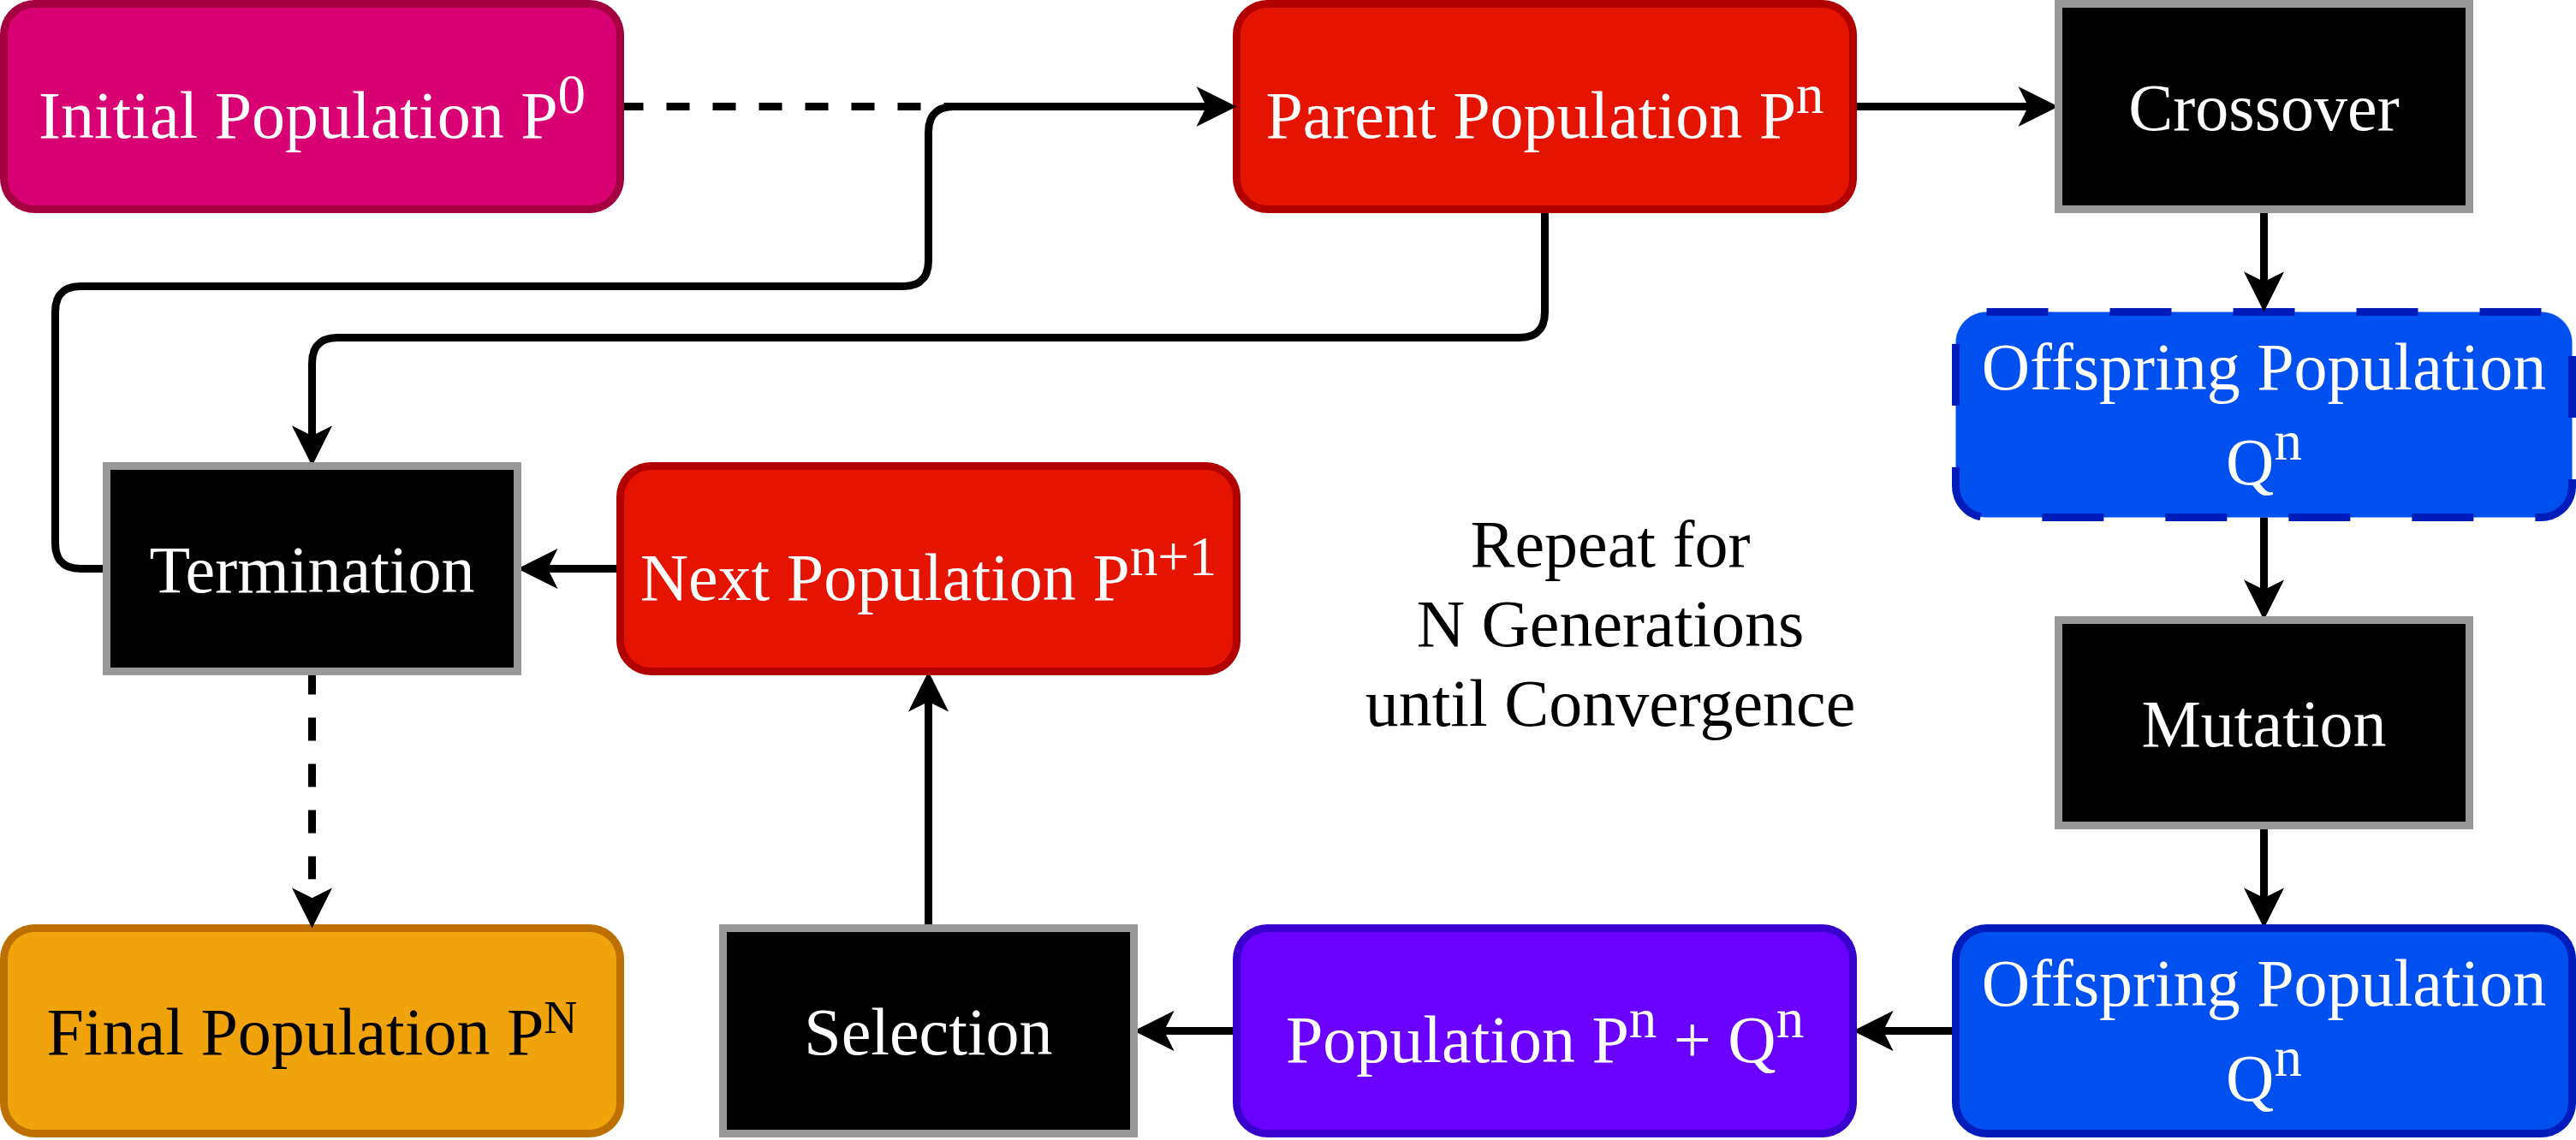
\includegraphics[width = \figurewidth]{figs/genetic_algorithm.png}
	\caption{}
	\label{fig:ga_schematic}
\end{figure}

%\begin{multicols}{2}

The operators used in \gls{ga} are Crossover, Mutation, Selection, and Termination. These operators take a population of solutions as inputs and return a population of solutions as outputs. \gls{ga} operators are defined in detail as follows:

\begin{description}
	\item[Crossover] The crossover operator batches population $P^n$ of size $M$ into pairs. Each pair begets two child solutions with each parent contributing roughly half of the genes of each child. This results in a child population $Q^n$ of size $M$.
	\item[Mutation] The mutation operator iterates through $Q^n$ and randomly resets the value of genes with a given probability.
	\item[Selection] The selection operator serves to determine which solutions of the combined population $P^n \cup Q^n$ will form $P^{n + 1}$.
	\item[Termination] The termination operator determines whether or not to produce another generation. Termination should occur after convergence.
\end{description}

\gls{ga} allows for the solution of an integer or mixed-integer problem without computing every possible combination of integer values. While optimal solvers are guaranteed to find the global optimum (subject to tolerances) \gls{ga} is not. \gls{ga} does not allow for computation of the optimality gap at any time, including at convergence. The likelihood of \gls{ga} arriving at the optimum increases asymptotically with the ratio of $M$ to the number of genes (variables) in $U$.

\subsection{Non-dominated Sorting Genetic Algorithm}

Extending \gls{ga} to \gls{moo} requires very little adjustment of the baseline method. Crossover, mutation, and termination operators remain unchanged. Only the selection operator is altered. Classically, the fitness of solution $U_i$ is determined by the objective function $J = F(U)$. A \gls{moo} problem is defined by a set of objective functions $\hat{F} = \{F_0, F_1, \dots, F_K\}$ which are not weighted relative to one-another and may be contradictory. Evaluating such functions relative to one-another requires introducing the concepts of Non-Domination and Crowding-Distance.

\subsubsection{Non-domination}

Solution $U_i$ dominates solution $U_j$ if and only if $F_k(U_i) \leq F_k(U_j)$ for all $F_k \in  \hat{F}$ and there exists some $\hat{F}' \in  \hat{F}$ where $F'_k(U_i) < F'_k(U_j)$ for all $F'_k \in  \hat{F}'$. In other words, $U_i$ dominates $U_j$ when $U_i$ is at least good in all aspects and better in at least one aspect. In this case, a rational decision maker, when presented with $U_i$ and $U_j$, will always pick $U_i$ regardless of personal priorities. The opposite condition is non-domination which occurs wherever the conditions of domination are not met. Non-domination is common with contradictory objectives such as price and quality. In this case, rational decision makers may disagree based on personal preference, even with identical information. 

A domination front is a set of solutions of the same domination rank. The first front are all solutions which are not dominated by any other solution. Unless all solutions are included in the first front, removing the first front is guaranteed to produce an new non-dominated front which can be called the second front. This process can be repeated until all solutions are assigned to a front as shown in Figure \ref{fig:non_dom_sort}. The rank of a solution is determined by its front and is the primary metric of selection.

\begin{figure}[H]
	\centering
	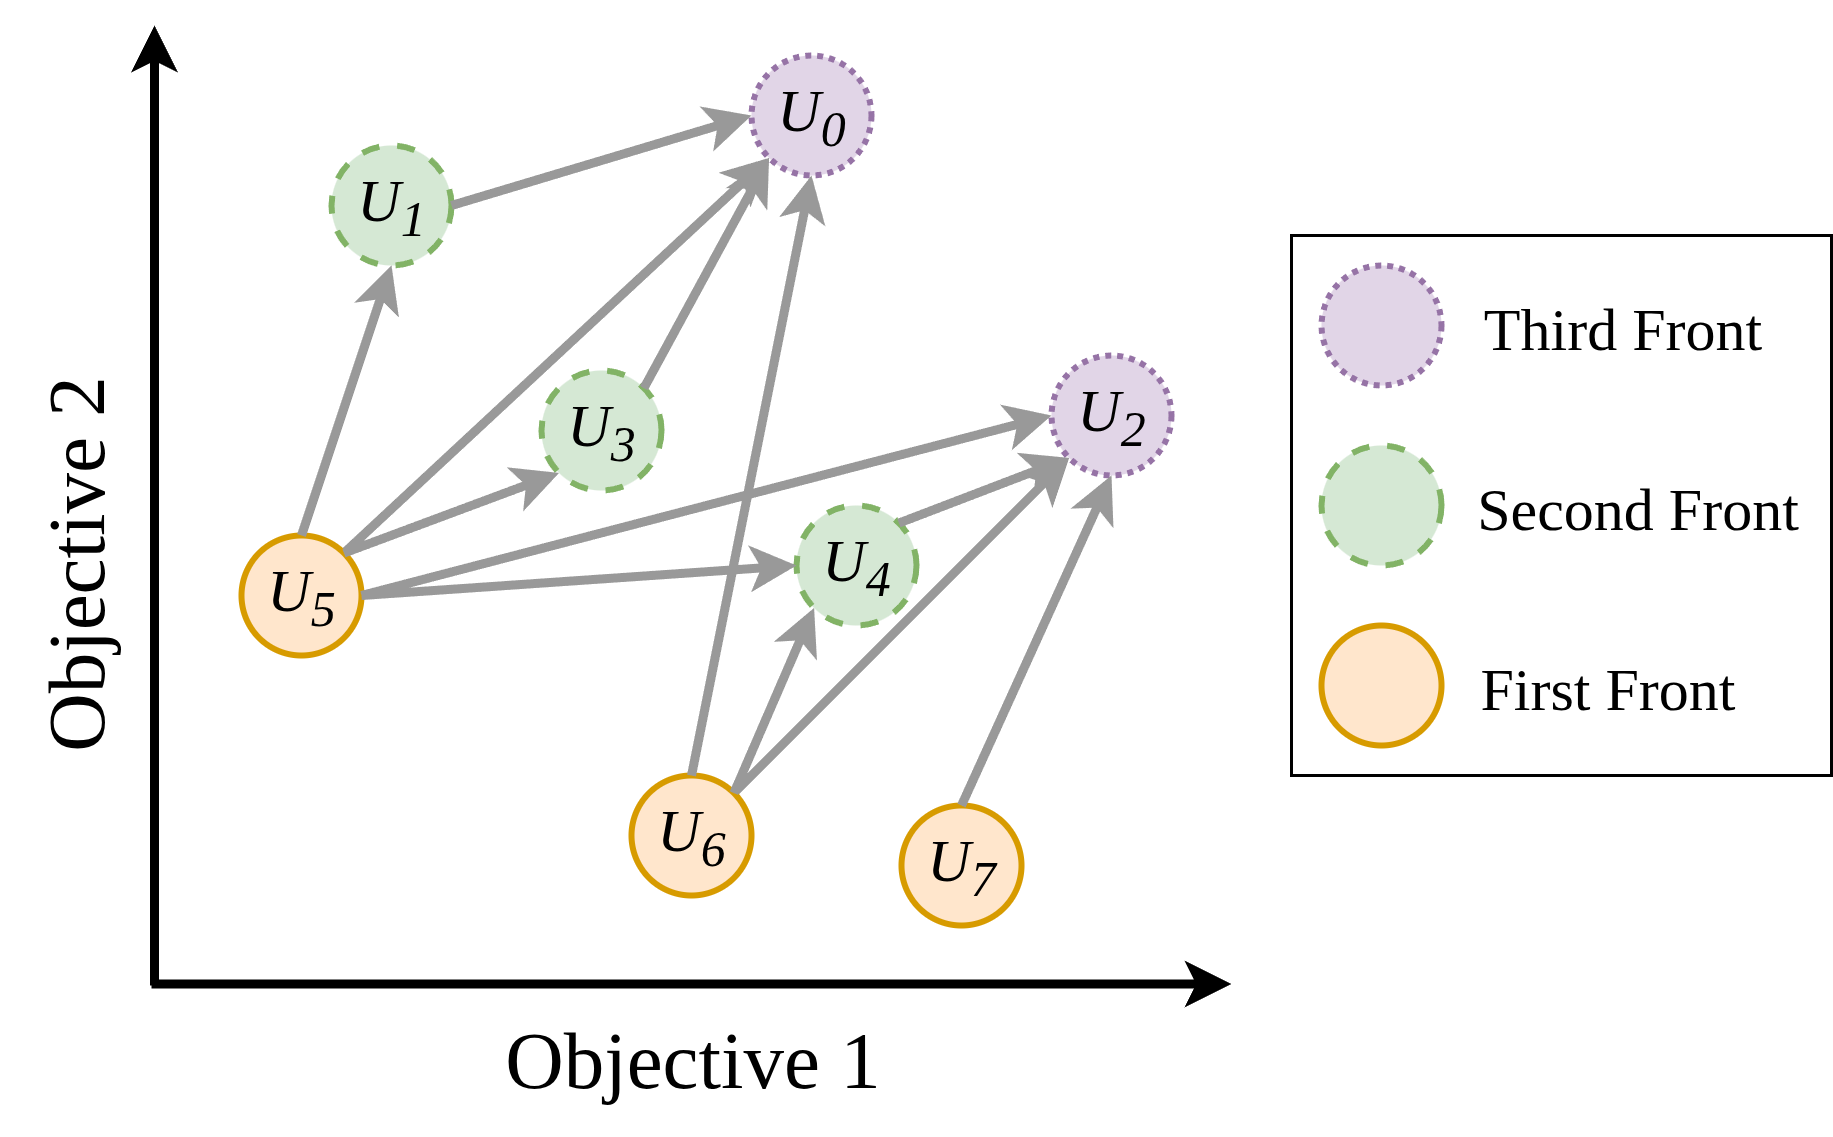
\includegraphics[width = \figurewidth]{figs/non-domination.png}
	\caption{Non-Domination Fronts}
	\label{fig:non_dom_sort}
\end{figure}

\subsubsection{Crowding-Distance}

Many solutions will be of equivalent rank one will often need to pick between solutions of equal rank. When choosing between solutions of equivalent rank, the maintenance of field spread is prioritized. Contribution to field spread is captured in the Crowding-Distance ranking. Crowding-Distance measures the gap in the front which would appear if $U_i$ were removed. Those solutions with the highest resulting gap are prioritized for selection. Each front must have two extrema for each objective. Extrema are awarded a crowding-distance of infinity. Crowding-distance ranking is demonstrated in Figure \ref{fig:crowding_distance}.

\begin{figure}[H]
	\centering
	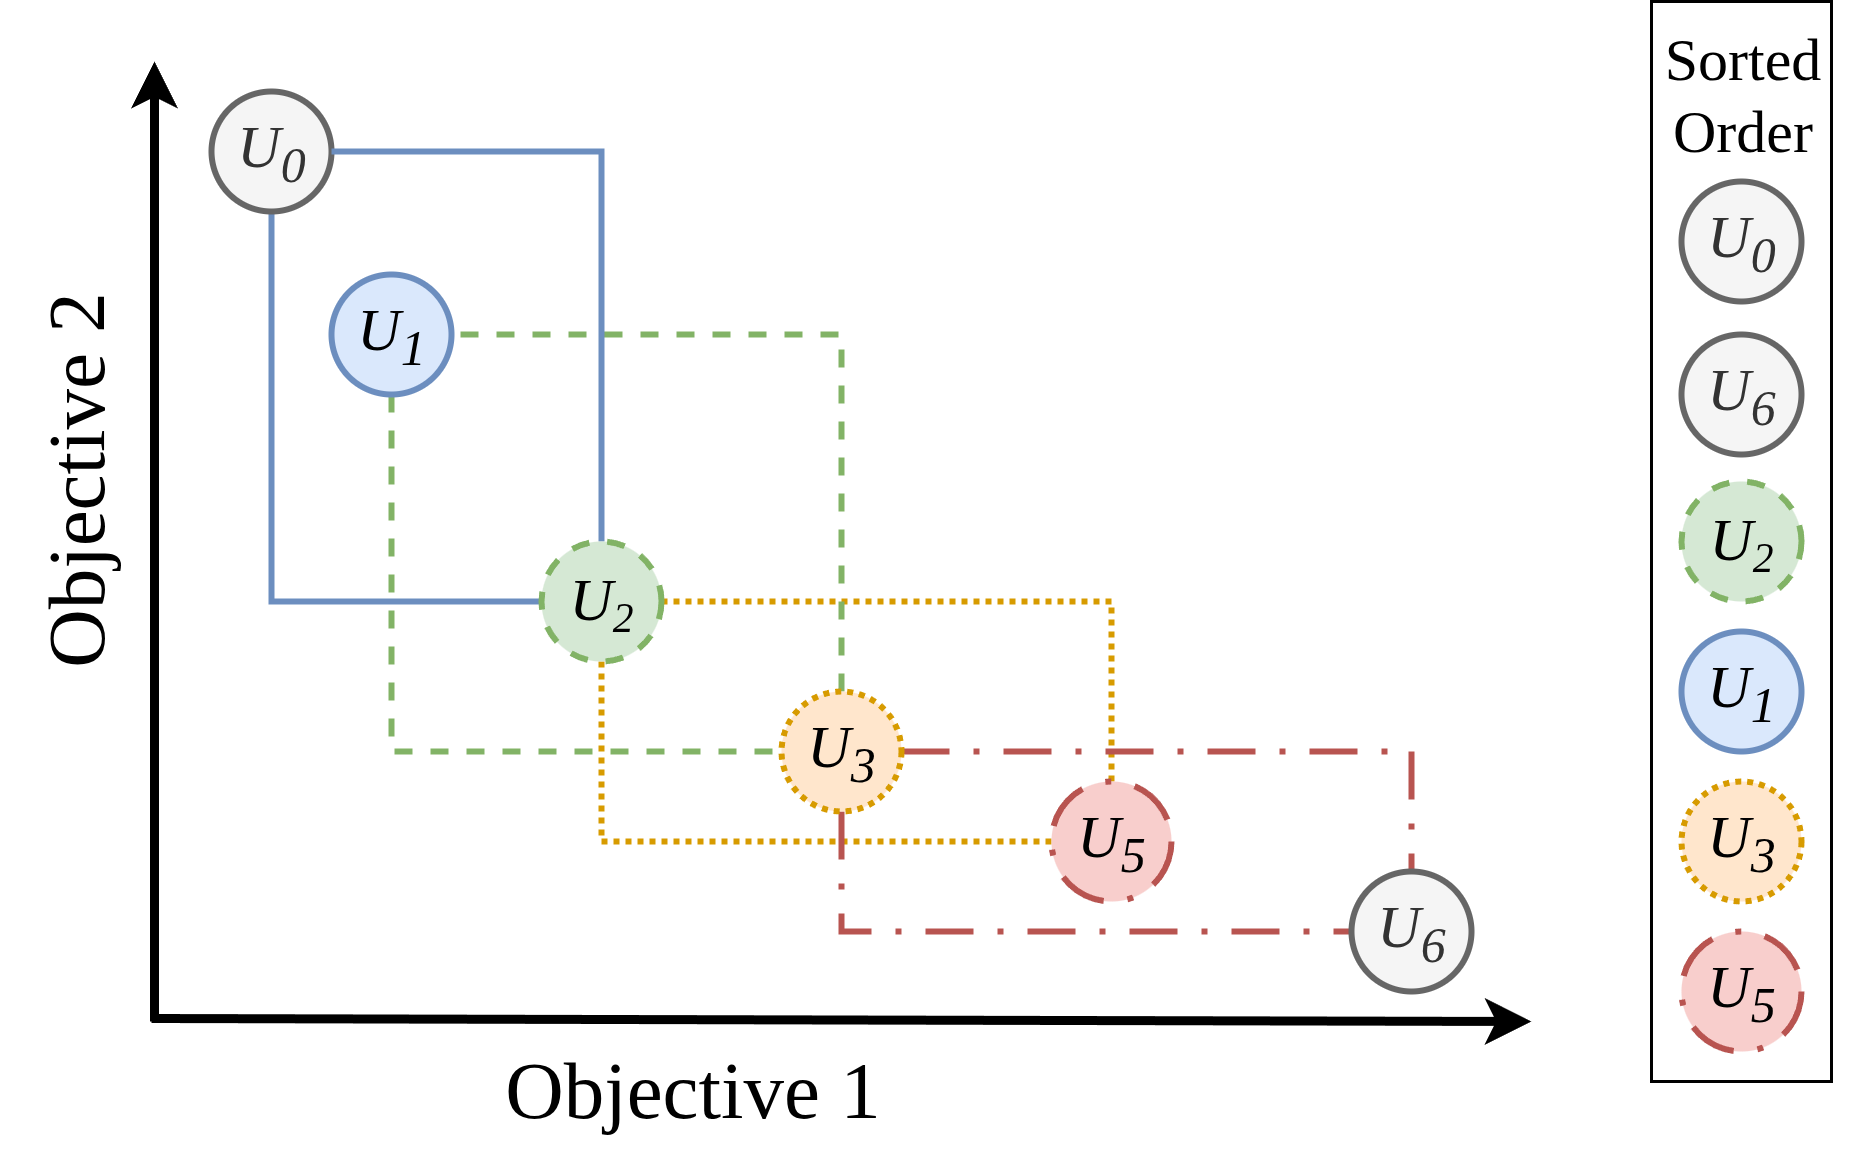
\includegraphics[width = \figurewidth]{figs/crowding-distance_1.png}
	\caption{Example crowding distance ranking. $U_0$ and $U_6$ are given a score of infinity as they are extrema. The remaining points are sorted in descending order based on the size of gap that would be created by their removal.}
	\label{fig:crowding_distance}
\end{figure}

\subsubsection{Selection}

\gls{nsga} calls for Elitist selection. From a combined population of $2 M$ solutions, the best $M$ solutions form the next generation. This is accomplished as follows. First, the solutions of the combined population $P^n \cup Q^n$ are ranked. Iterating through fronts in order, if the size of a front is less than $M - |P^{n + 1}|$ then the entire front is added to $P^{n + 1}$. If the size of the front is greater than $M - |P^{n + 1}|$, then the solutions in front are sorted for crowding-distance and solutions are added in order until $|P^{n + 1}| = M$.

\subsection{Defining the \gls{vsfmp}}

The \gls{vsfmp} concerns the optimization of strategic purchasing decisions for a bus fleet or other vehicle fleet with rigidly scheduled service trips. The problem is solved by finding an assignment of vehicles to service trips and supply events and an assignment of supply equipment to supply events. The assignment must account for the cost and feasibility of transitioning from one service trip or supply event to another. Purchasing and installing equipment incurs up-front costs which scale with the amount purchased while operating costs scales with time worked and energy expended. The method presented is generic and specific cost functions will be provided for case studies.

\subsection{Encoding the \gls{vsfmp}}\label{sec:ebrp}

Posing the \gls{vsfmp} for \gls{ga} requires encoding the problem onto chromosomes. This is non-trivial due to the nature of the problem. Previous schema are presented in \cite{Rogge_2018_AE, Li_2020_JAT, Yao_2020_SCS}. Where \cite{Li_2020_JAT} is a straightforward implementation, the others reformulate the \gls{vsfmp} to better fit \gls{ga}. The approach of \cite{Rogge_2018_AE} is to group service trips into blocks (tours) and solve a simplified \gls{milp} while the approach of \cite{Yao_2020_SCS} is to encode trip order into chromosomes and use a heuristic assignment method. The proposed method draws inspiration from both. First a graphical structure is devised which serves as the chromosomes indirectly encoding vehicle tours and allowing for straightforward crossover and mutation. Following this, an assignment heuristic is utilized for the reduced problem. This approach provides a more direct link between genetic material and fitness compared to \cite{Yao_2020_SCS} and a more direct crossover and mutation compared to \cite{Rogge_2018_AE}. The method is also generic and inherently suited for \gls{moo}.

The encoding scheme is built around three structures. The first structure is the Successors Graph which stores the successor activity for each trip (another trip or return to depot). The second is the Vehicle Type Map which assigns a vehicle type to each trip. The third is the Port Type Map which assigns a supply port type to each trip. These structures constitute the genetic material. The structures must be co-optimized as there is substantial interaction between them.

\subsubsection{Successors}

A bus network schedule is a set of trips $V$ where each trip is defined by start and finish times and locations and energy requirements. Given knowledge of the time required to transition between route terminals and depots, it is possible to construct Trips Graph $G = \{V \cup D, E\}$ where $D$ contains all depots and $E$ contains all possible transit legs.

Tours may be stored by storing the successor activity to each trip. For a valid tours assignment, all trips $v_i \in V$ must have exactly one successor. This successor may be another trip or a depot. Depots $d_i \in D$ may have many successors but it is not necessary to store these. The predecessor-successor links form the edges of a directed Successors Graph $G^S = \{V \cup D, S\}$ where $S \in E$ are the edges which form the tours. Edges in $S$ may only originate with a trip in $V$ but may terminate with a trip in $V$ or a depot in $D$. There are many possible permutations of $S$ for any realistically scaled $G$. The set of possible permutations of $S$ is $\hat{S}$ and much of the work of solving the \gls{vsfmp} is finding the subset of $\hat{S}$ that corresponds the Pareto Front in an efficient manner. $S^T = \{i\ \forall\ (i, j) \in S\}$ is the set of tail nodes for the edges in $S$ and $S^H = \{j\ \forall\ (i, j) \in S\}$ is the set of head nodes for the edges in $S$. $S^T$ must contain all trips in $V$ but $S^H$ need not contain all trips in $V$.

For each $S_i \in \hat{S}$ there is a corresponding Predecessors Set $\Pi_i$ whose edges are $\{(j, i)\ \forall\ (i, j) \in S\}$ such that the graph formed from the combination of $S^i$ and $\Pi^i$ is undirected. $\Pi^i$ is used to recover tours. Starting from depots, \gls{bfs} is used to recover all tours up to the point that predecessors are exhausted. Since tours must start and finish at the same depot, each tour starts at the same depot at which it finishes.

Consider the simple Trips Graph shown in Figure \ref{fig:trips_graph}. The simple Trips Graph defines a network which operates two routes for three trips each.

\begin{figure}[H]
	\centering
	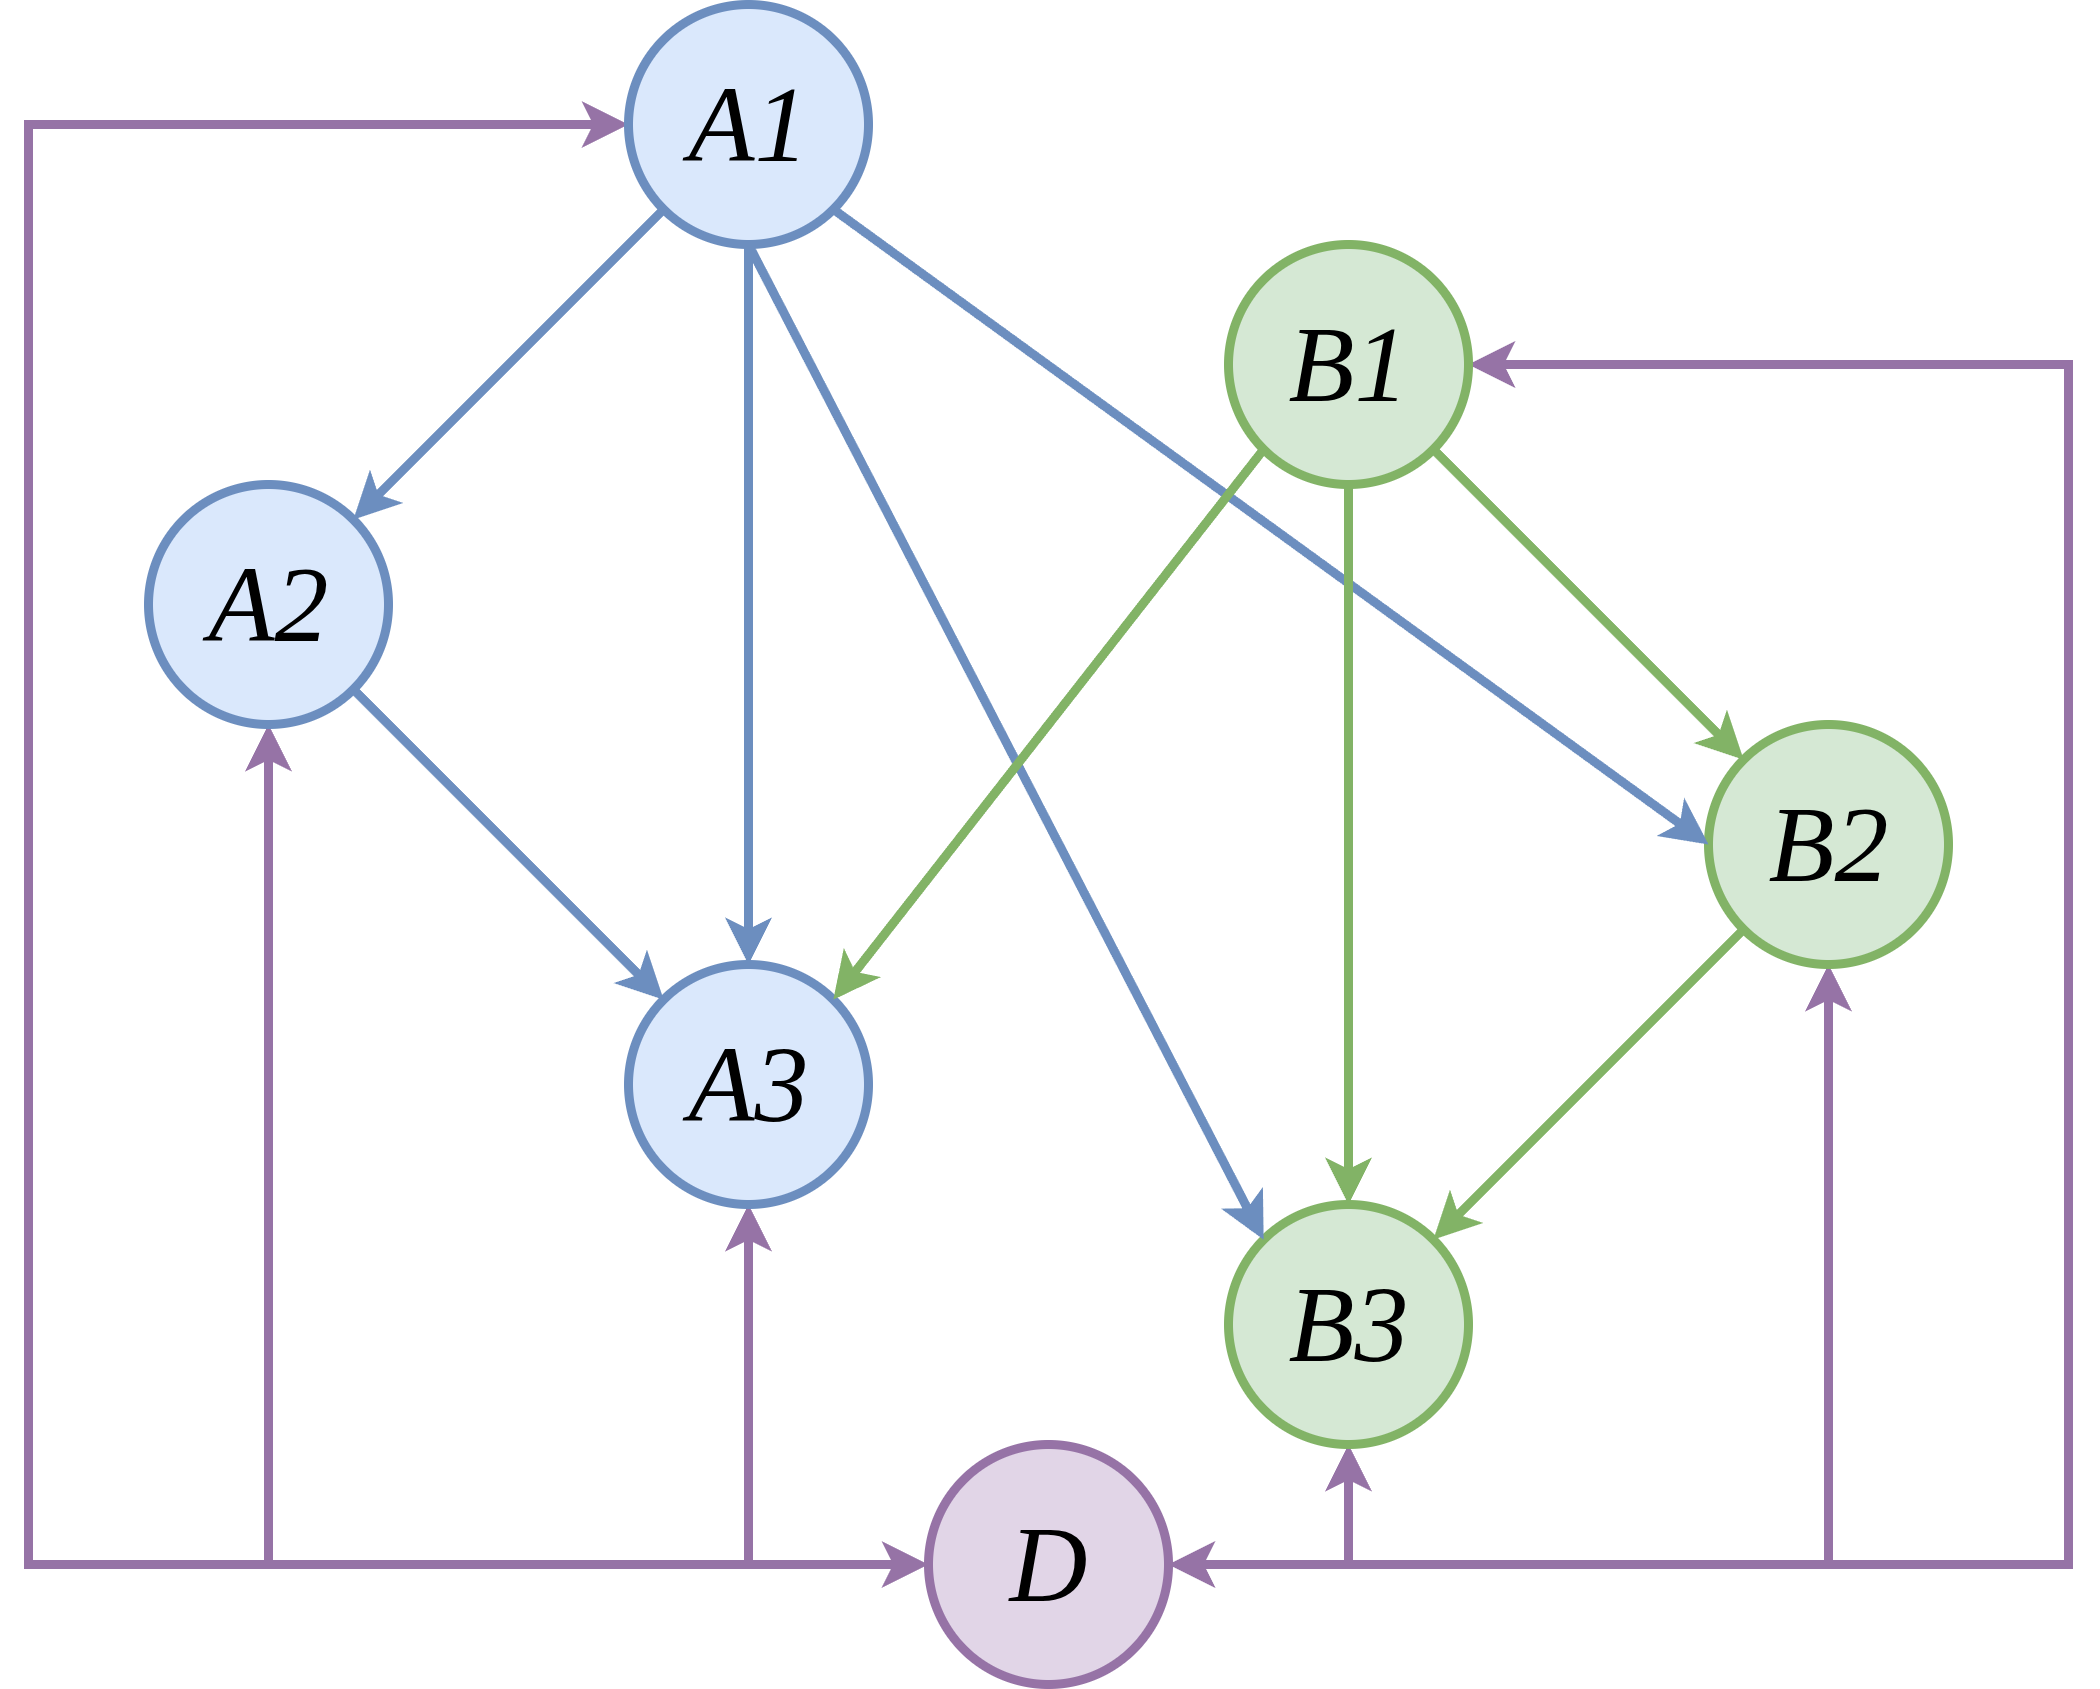
\includegraphics[width = .5\linewidth]{figs/trips_graph.png}
	\caption{}
	\label{fig:trips_graph}
\end{figure}

A valid Successors and the resulting Predecessors are provided in Figure \ref{fig:successors_predecessors}.

\begin{figure}[H]
	\centering
	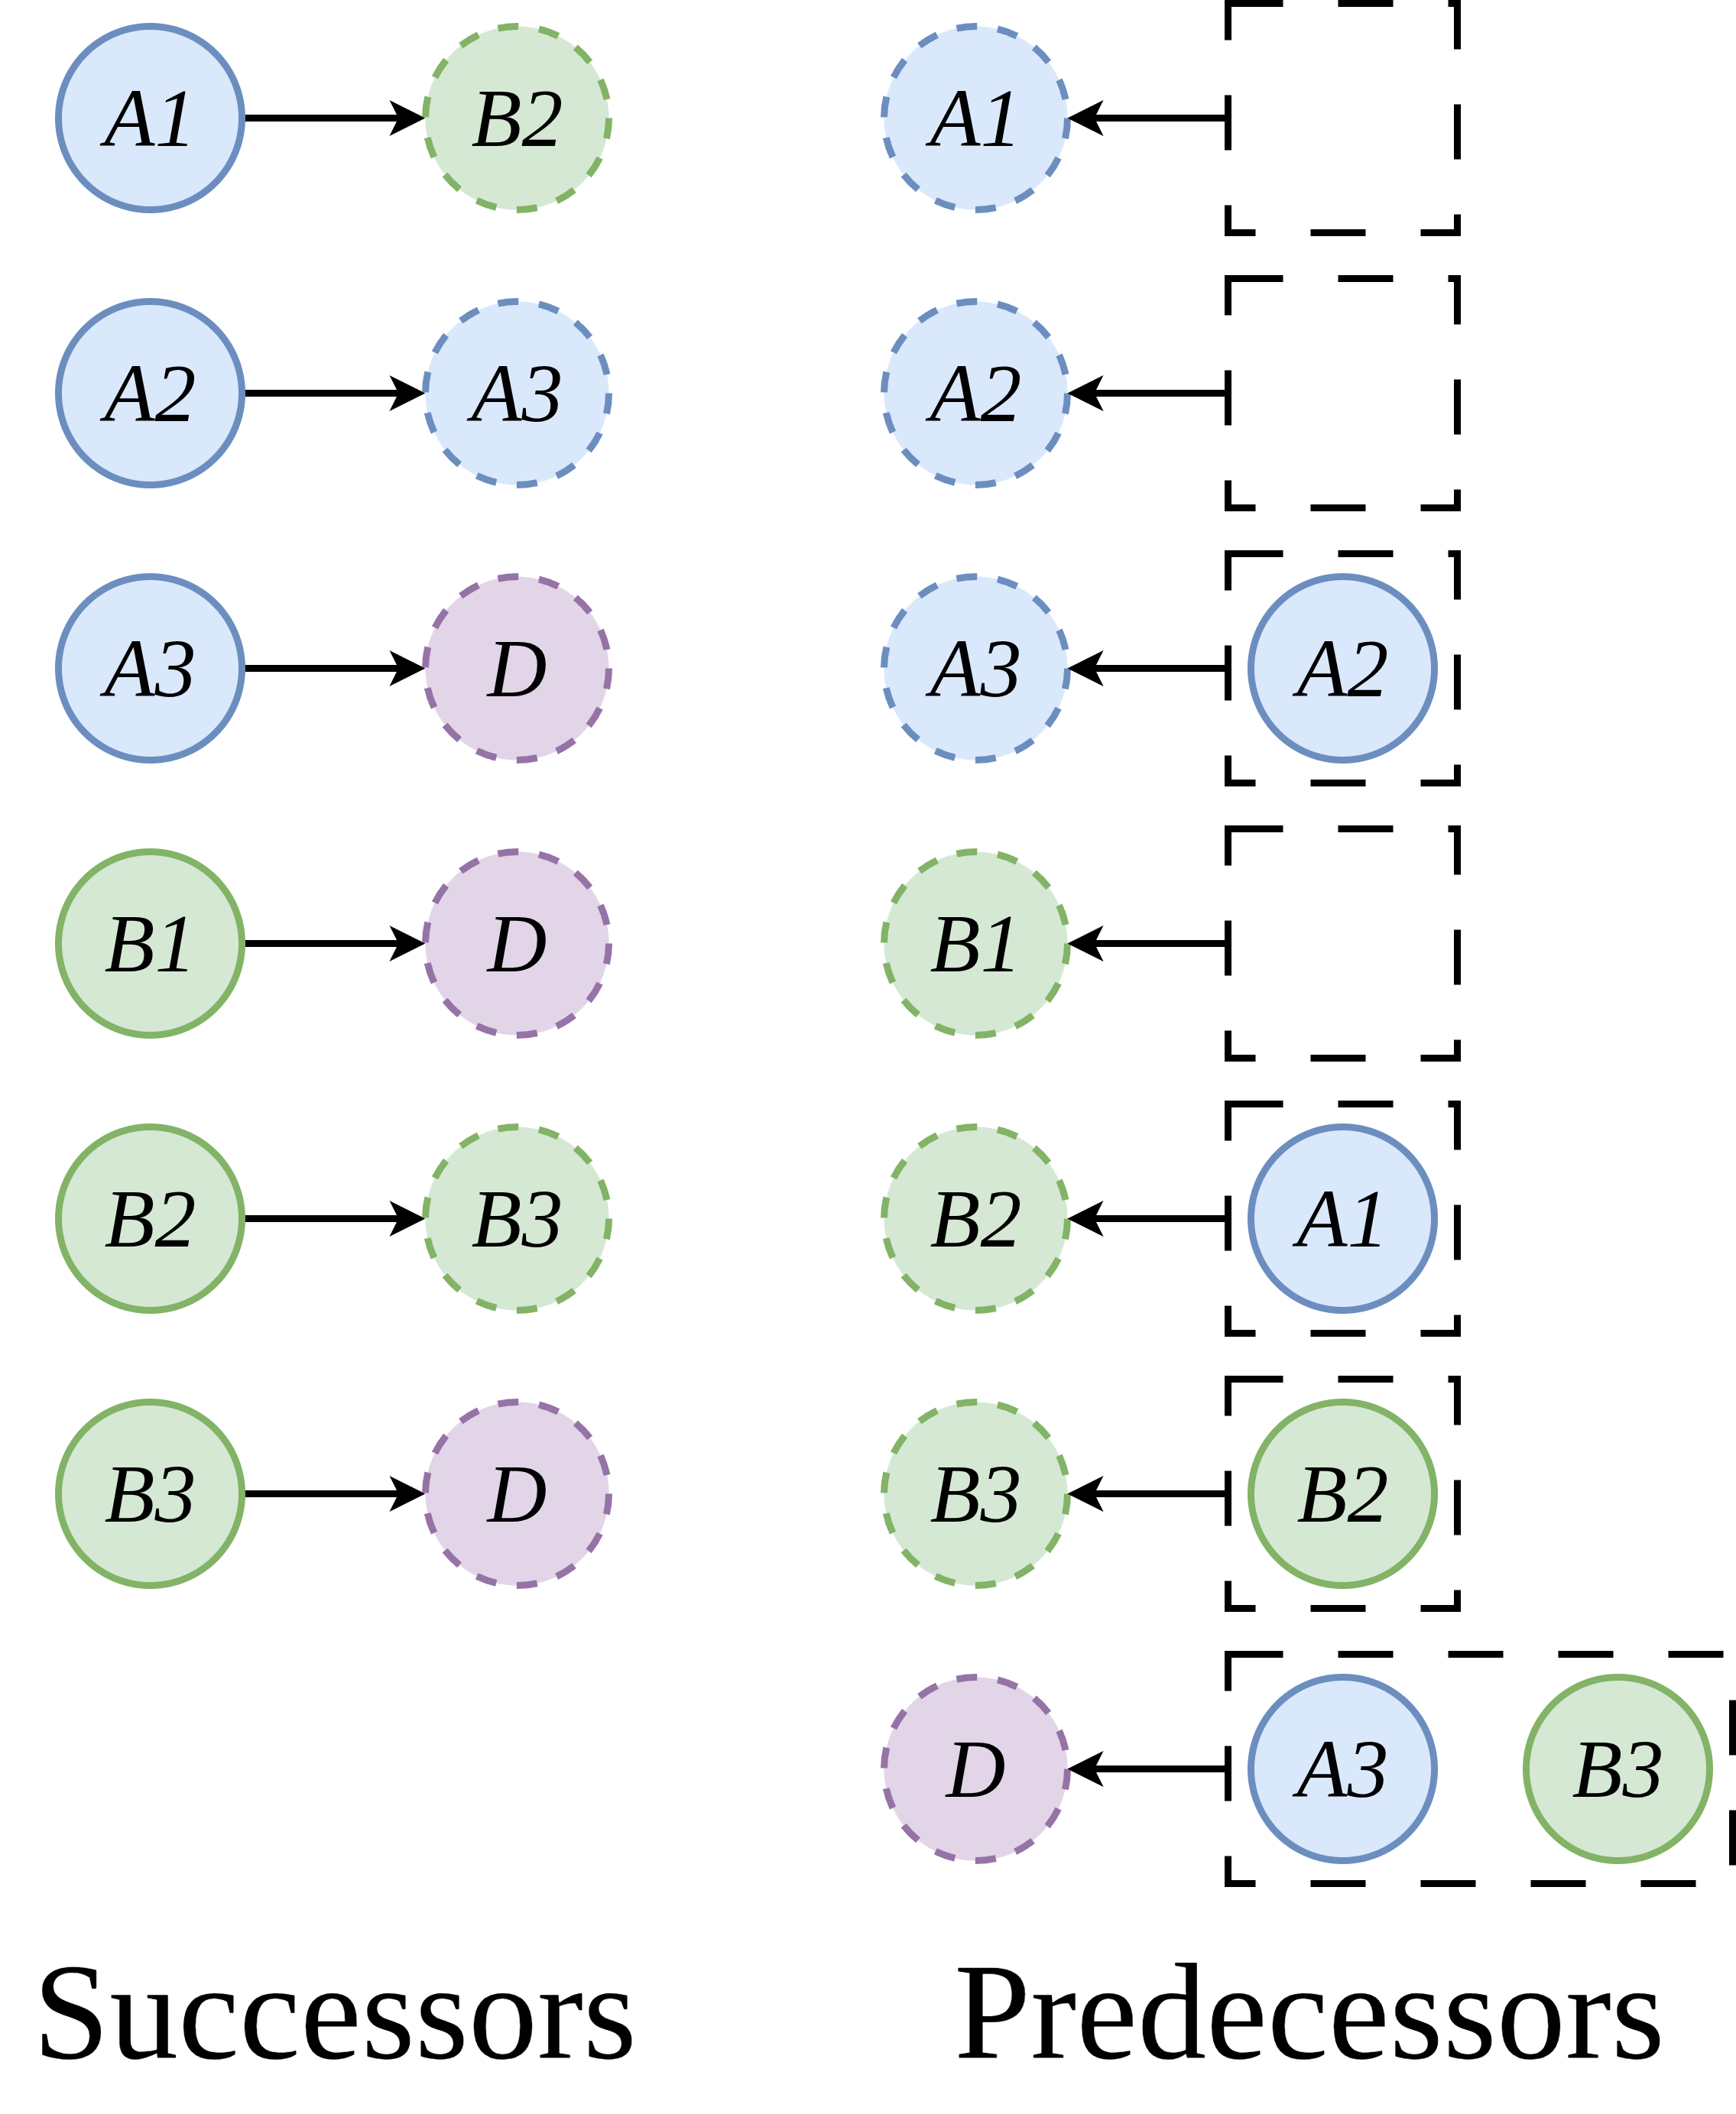
\includegraphics[width = .5\linewidth]{figs/successors_predecessors.png}
	\caption{}
	\label{fig:successors_predecessors}
\end{figure}

Which leads to the set of tours shown in Figure \ref{fig:tours}.

\begin{figure}[H]
	\centering
	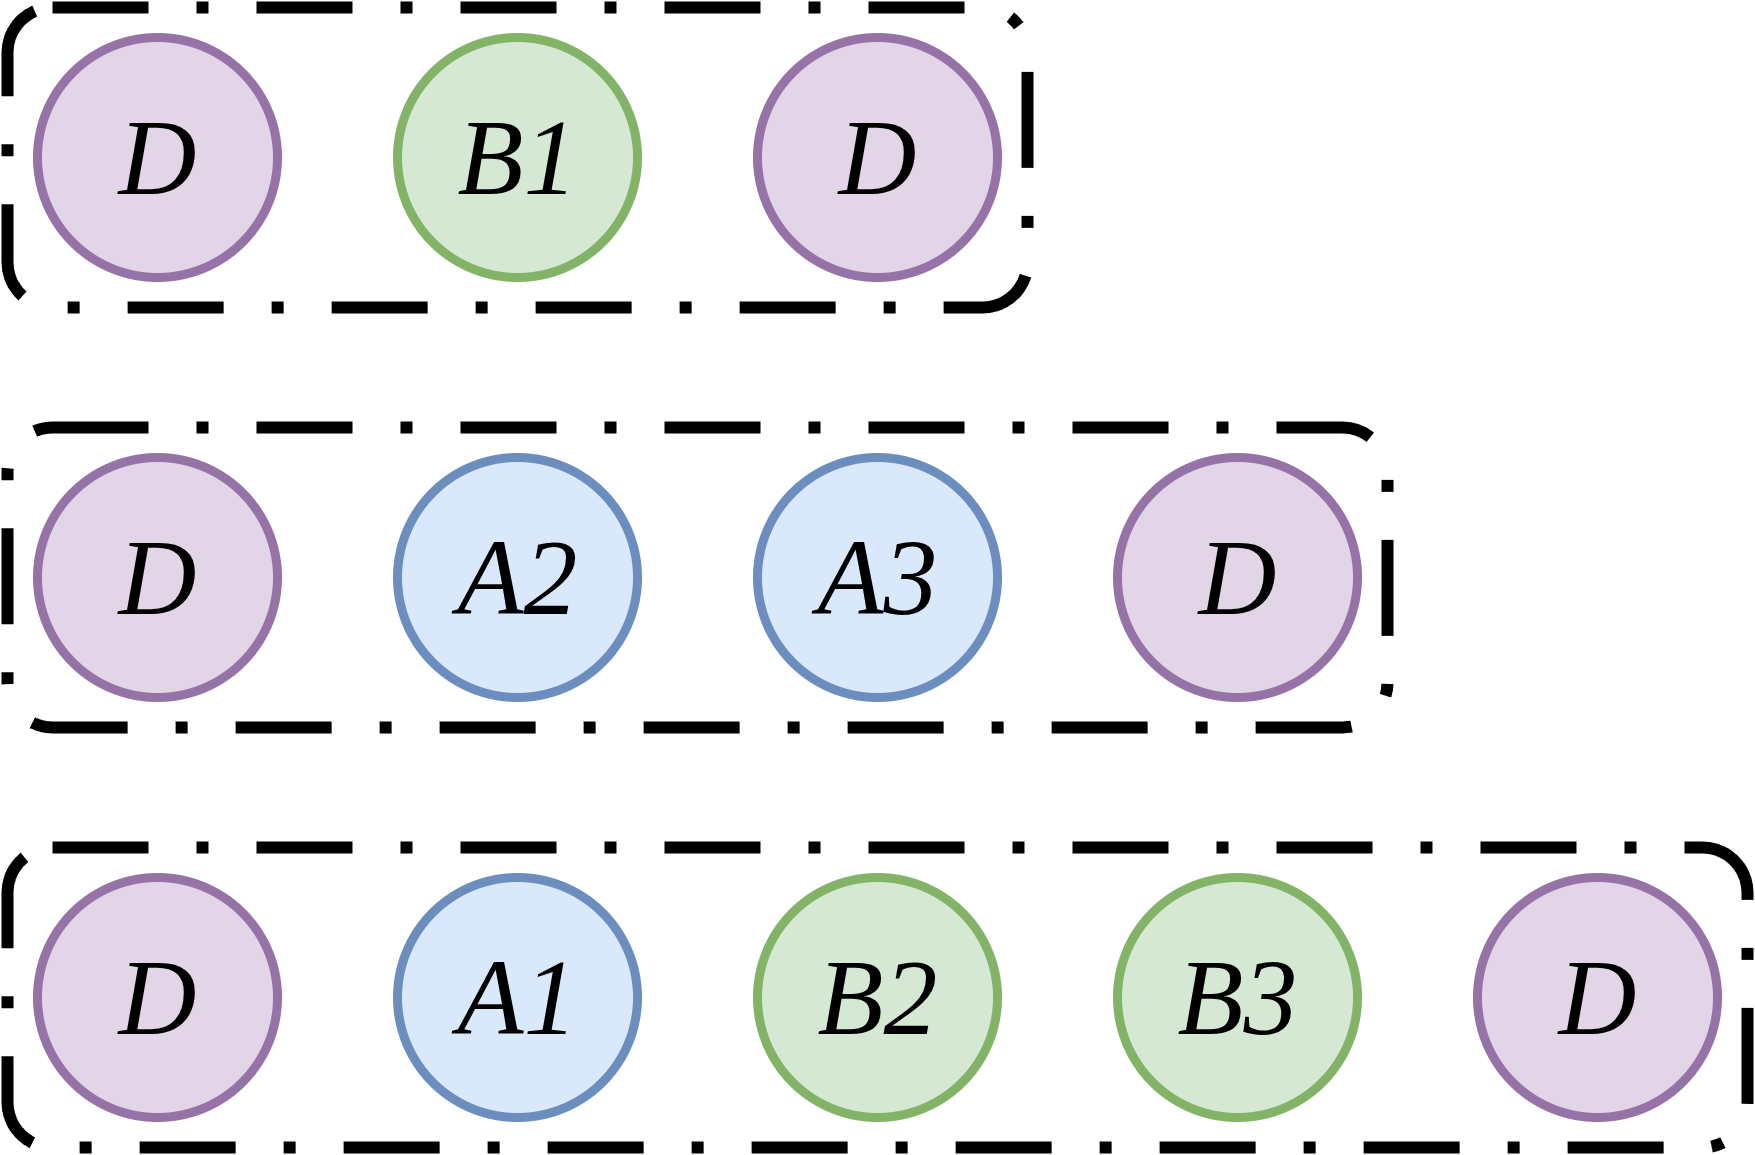
\includegraphics[width = .5\linewidth]{figs/tours.png}
	\caption{}
	\label{fig:tours}
\end{figure}

The Successors structure leads directly to the tours. Although this encoding is more memory intensive than a simple ordering it allows for simple and robust Crossover and Mutation operators.

\subsubsection{Vehicle Types}

The Vehicle Type Map is a simple map linking trips in $V$ to vehicle types in the set $B^V$ $A^V: V \rightarrow B^V$. Each trip in $V$ receives an assigned vehicle type in initial population generation. After tours are reconstructed, many tours will contain trips with multiple bus-type assignments. In this case, there is a "vote". If one bus type attains a plurality within the tour, the tour is assigned that bus type. Ties are broken by order of appearance. Following the vote, all trips in the tour are assigned the selected vehicle type. This process is shown in Figure \ref{fig:voting}.

\begin{figure}[H]
	\centering
	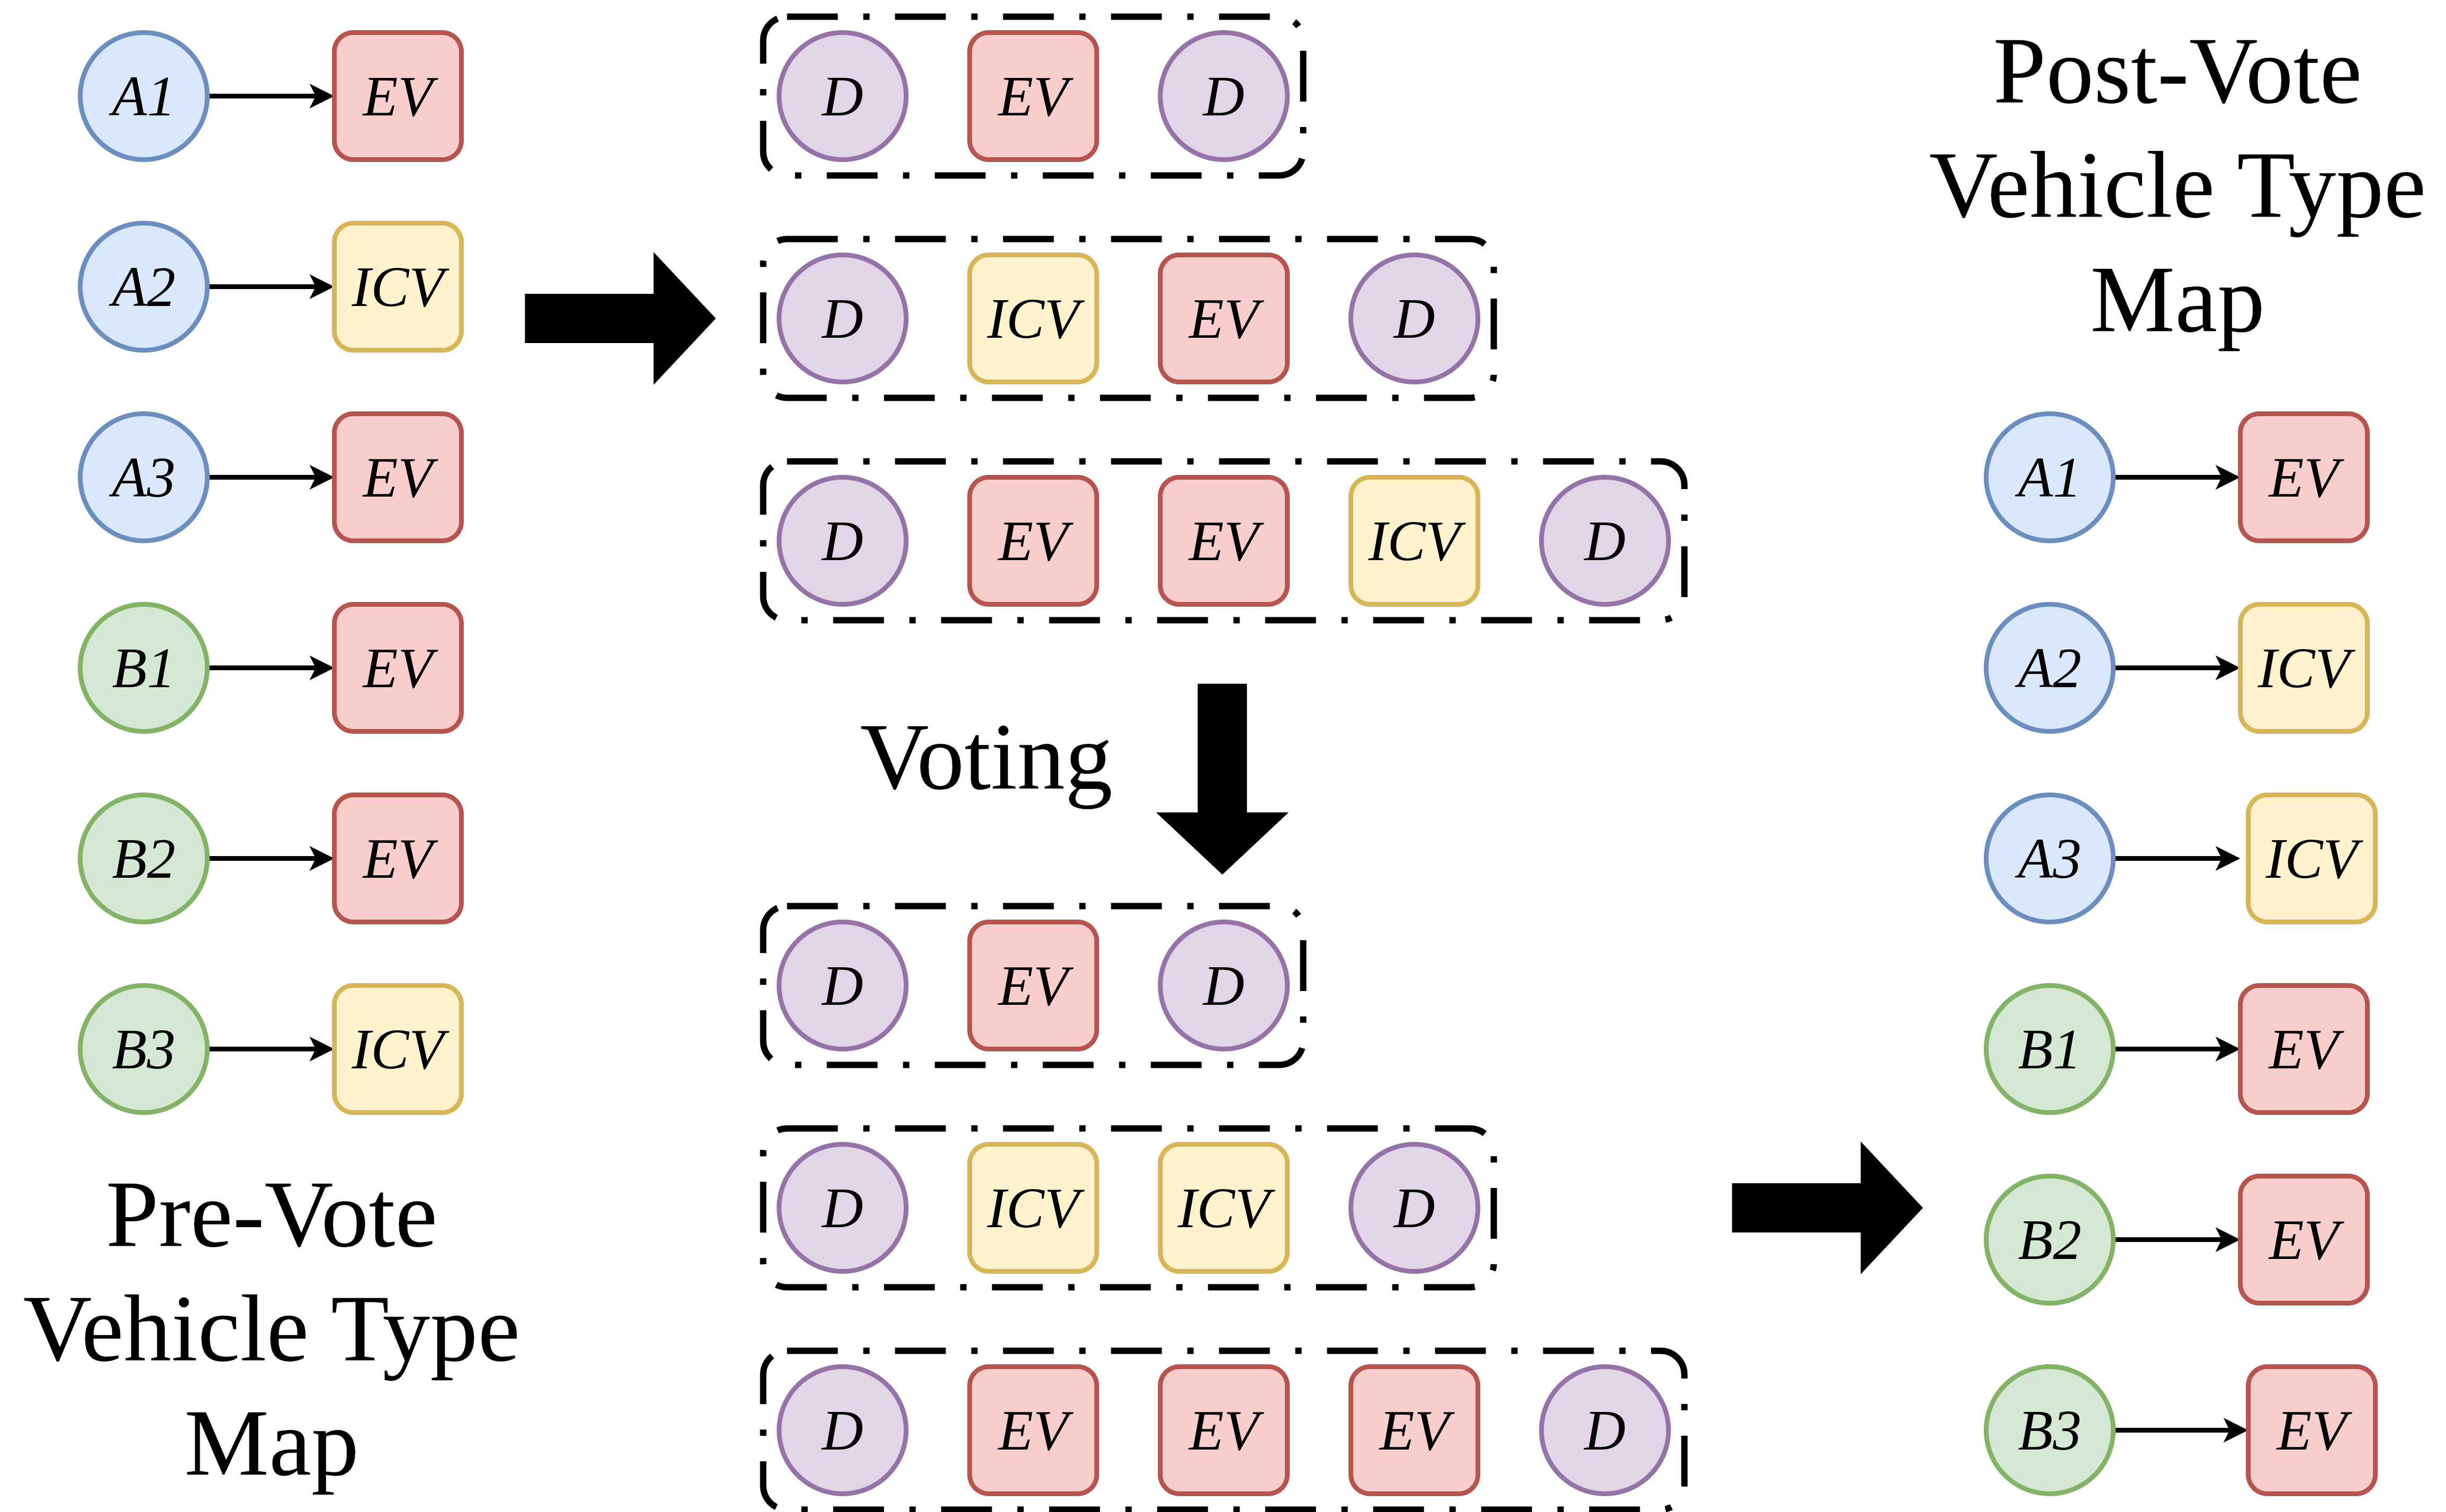
\includegraphics[width = \linewidth]{figs/voting.png}
	\caption{}
	\label{fig:voting}
\end{figure}

\subsubsection{Port Types}

The Port Type map $B^P$ $A^P: V \rightarrow B^P$ functions similarly to the Vehicle Type map. When the Port Type map is initialized, each assignment is a valid assignment for the type of vehicle assigned to the same trip. When the vehicle type for a tour is determined, the port type for the tour is the predominant port type among the vehicles of the selected vehicle type included in the tour. Thus the port type selected for a tour will always be compatible with the vehicle type.

\subsection{Assignment Heuristic}

Having formed the tours and determined vehicle and port types, the problem becomes an assignment problem. This assignment determines which specific bus within a given type will serve a specific tour and which specific port will serve the succeeding supply event.

First, following vehicle type assignment, it is possible that some tours will be infeasible for the vehicle type chosen. In this case, the tours in question are subdivided into two tours with this process repeating until all tours are feasible. Individual vehicles are assigned to tours based on the assigned vehicle type using the heuristic defined in Figure \ref{fig:bus_assignment}.

%\end{multicols}
\begin{figure}[H]
	\centering
	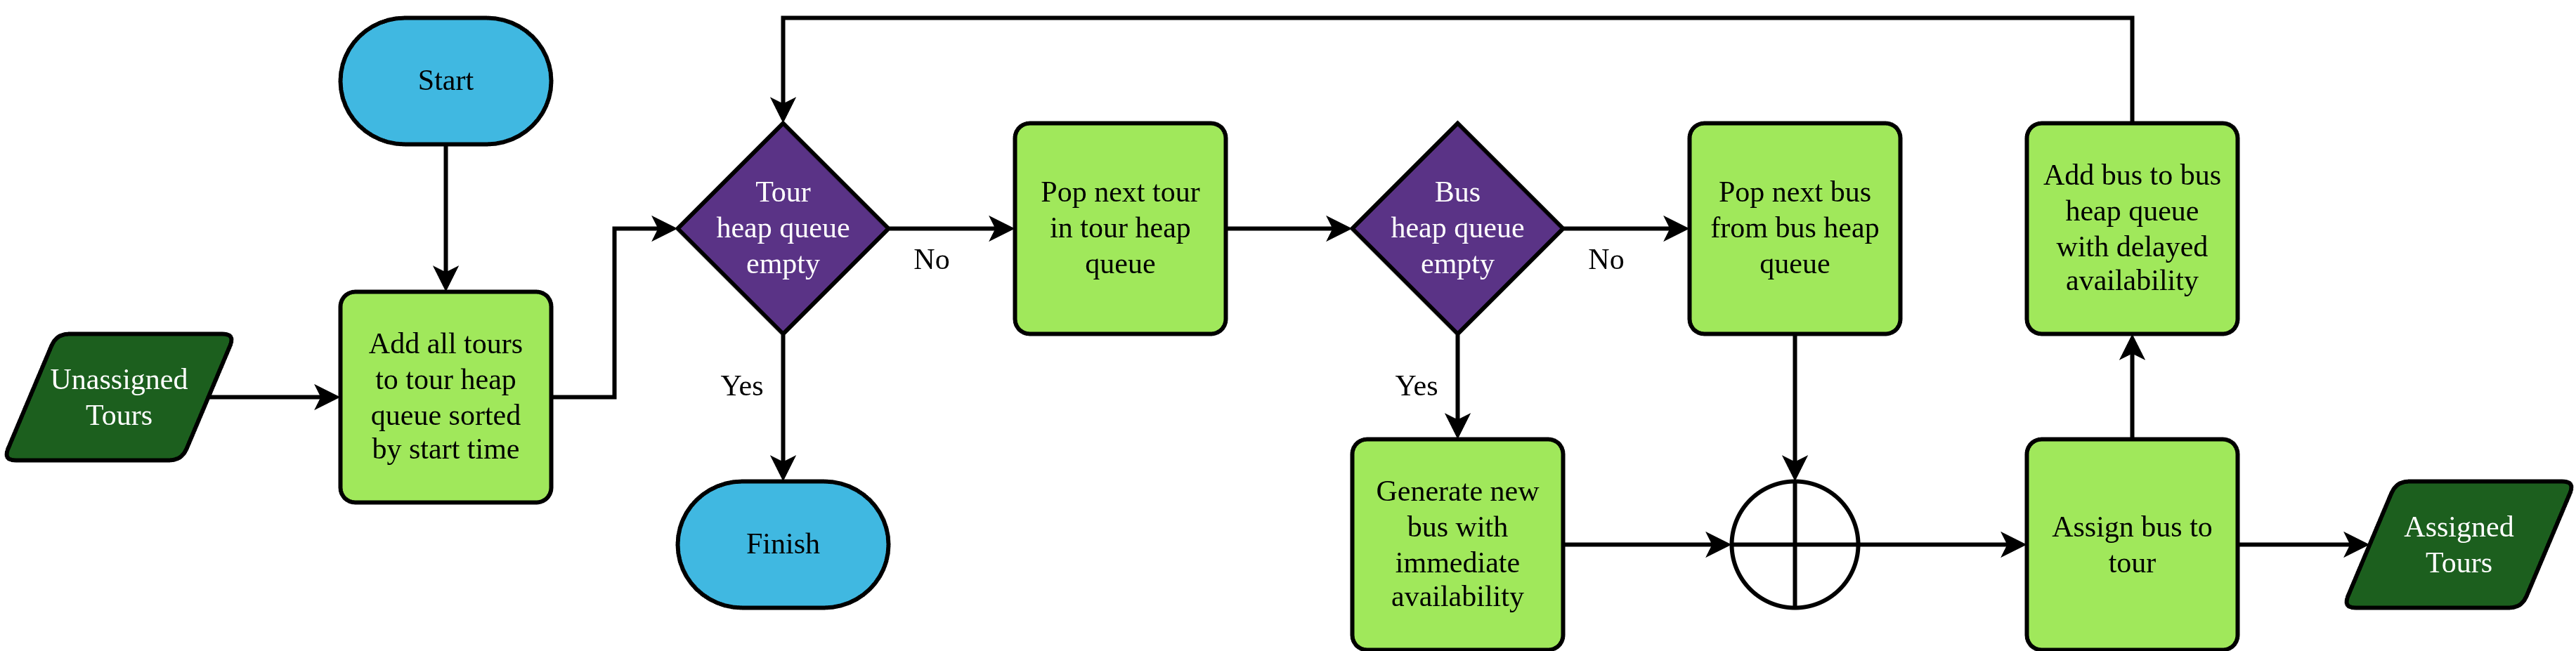
\includegraphics[width = \linewidth]{figs/bus_assignment_1.png}
	\caption{}
	\label{fig:bus_assignment}
\end{figure}
%\begin{multicols}{2}

The process shown in Figure \ref{fig:bus_assignment} pertains to a fleet of a single vehicle type but can be easily extended to multiple vehicle types by implementing a separate queue fo each vehicle type and choosing from the appropriate queue. The heuristic will result in an individual vehicle assigned to each tour and a required number of vehicles for each type.

Having assigned individual vehicles to tours, supply equipment can be assigned to the supply events which follow the tours. Each tour which terminates at a depot with a supply station will be followed by a supply event (charging or fueling) which must be completed before the vehicle can perform another tour. Supply ports are added and assigned to supply events in a similar manner to the vehicle assignment. The main differences are that where tours are sorted by start time, supply events are sorted by finish time.

\subsection{Custom Genetic Operators}

The unique encoding scheme introduced in Section \ref{sec:ebrp} requires custom genetic operators to function. The specific forms of initial population generation and the Crossover and Mutation operators required are discussed in the following sections.

\subsubsection{Initial Population}

The initial population is generated by generating $M$ random configurations of $S$ and $A$. Generating a valid random configuration of $S$ requires that each trip in $V$ have exactly one predecessor and successor in $V \cup D$. This is accomplished by iterating through the trips in $V$ in random order and, for each trip, randomly choosing a successor from the set of possible successor trips and depots. Each time a successor is assigned the successor trip is no longer able to be selected for any other trip. $A$ is generated by random selection of vehicle types in $B$ for each trip in $V$. The Vehicle Type and Port Type maps are also randomly generated. For each trip in $V$, a vehicle type is selected from a weighted distribution among the types in $B^V$ and a valid port for said vehicle type is randomly selected from $B^P$. 

\subsubsection{Crossover and Mutation}

Crossover is accomplished by the exchange of genetic material among randomly selected pairs of parents from $P^n$ with each parent paired exactly once. For parents $a$ and $b$ children $c$ and $d$ are formed by the crossover process. Child $c$ is formed by copying parent $a$ and subsequently incorporating selected genetic material from parent $b$. Child $d$ is formed by copying parent $b$ and subsequently incorporating selected genetic material from parent $a$. The contribution to child $c$ from parent $a$ is referred to as the original material and the contribution from parent $b$ is referred to as the crossover material and \textit{vice versa} for child $d$. In order to minimize duplicated work the Crossover and Mutation operators are merged. If the mutation probability is greater than zero, randomly selected genes are changed within the crossover material before crossover happens. Crossover and Mutation are accomplished differently for Successors and Vehicle/Port Types.

\paragraph{Successors} Crossover of successors is accomplished by the random swapping of edges in the Successors Graph among pairs of parents from $P^n$. As the Successors Set contains an edge for each trip in $V$, each $S \in \hat{S}$ will have the same number of edges with the same tail nodes. Edges are selected for crossover randomly with a probability of $\phi^c$ which is $0.5$ by default. Mutation occurs with probability of $\phi^m$ and involves swapping the selected edge with another edge in $E$ with the same tail node. On its own, this will often create a situation where one node serves as successor to multiple other nodes, thus appearing in multiple tours. This is invalid and requires adjustment of $S$. Consider the insertion of $(t, h)$ from $S_b$ into $S_a$. $S_a$ will contain an edge $(t, h')$ which contains the same tail node and, a possibly different head node. $S_a$ may also contain an edge $(t', h)$ which has the same head node as the inserted edge but a different tail node. This can create a conflict. The following operations are used depending on what potential conflicts exist.

\begin{description}
	\item[Clean Insert] If $(t', h) \notin S_a$ ($h$ is not the successor for any trip) then $(t, h)$ can replace $(t, h')$ without causing a conflict. In this case $h'$ no longer serves a a successor to any trip.
	\item[Replacement] If $(t', h) \in S_a$ ($h$ is the successor for another trip $t'$) and $(t', h')$ is not a possible edge then $(t, h')$ is dropped from $S_a$ and $S_a$ gets $(t, h)$. In this case $h'$ no longer serves a a successor to any trip and $t'$ no longer has a successor trip.
	\item[Swap] If $(t', h) \in S_a$ ($h$ is the successor for another trip $t'$) and $(t', h')$ is a possible edge then a swap occurs and $S_a$ gets $(t, h)$ and $(t', h')$.
\end{description}

\paragraph{Vehicle and Port Types} Each solution in $U_i \in P^n$ contains a unique vehicle type mapping $A^V$ and port type mapping $A^P$. Crossover is straightforward. A set of trips are designated for crossover and the vehicle types and port types are swapped between the parents. Vehicle and port types are swapped simultaneously and for the same selected trips in order to maintain valid port assignments.

\subsection{Constraint Handling}

It is possible for a valid solution to be in violation of some specified constraint. An example may be a limit on expenditures or fleet size. In this case, a compliant-first approach is used. Non-compliant solutions are given ranks which are higher than all compliant solutions. Thus, non-compliant solutions are able to be selected only if there are fewer than $M$ compliant solutions from $P^n + Q^n$.

\subsection{Termination}

A downside of \gls{ga} is that it is not possible to know whether or not a global optimum has been attained. Traditionally, convergence criteria are used for termination. For single-objective optimization, convergence can be determined by the evolution of the best or average value in the population. For Pareto optimization, this method can be misleading. Meaningful expansion of the Pareto front can manifest as no change ot the average or even a reversion. As such, the termination criteria used herein are a minimum number of generations $N^-$, a maximum number of generations $N^+$, and a child survival threshold. As the Pareto front advances, it becomes increasingly unlikely that child solutions will dominate their parents and, as such, be included in the subsequent generation. Thus, between the minimum and maximum number of generations, iteration terminates when fewer than a given number of child solutions survive to the next generation for a given number of consecutive generations.

\subsection{Run-Time Complexity}

The time-complexity of \gls{ga} and \gls{nsga} is known to scale as $O(MN)$ where $N$ is the number of generations and $M$ is the population size. Run-time is, thus, bounded by $O(MN^-)$ and $O(MN^+)$ which may be a large range. Because $N$ is not pre-determined and termination follows convergence the practical run-time is difficult to estimate.

Run-time is most meaningfully impacted by the scale of the Trips Graph $G$ including number of trips in $V$ and the number of feasible connections in $E$. This impact is felt in fitness evaluation, Crossover, and Mutation, and impacts the number of generations required for convergence $N$. Fitness evaluation requires finding tours which relies on \gls{bfs} thus scaling with $|V| + |E|$. All other operations including vehicle and port assignment scale with the number of tours and can be estimated as scaling with $|V|$. Crossover and Mutation require iterating through $S$ so they scale with $|V|$. Ultimately, the expected number of generations before convergence scales with the number of possible configurations of $S$ as well as the inverse of $M$. As will be demonstrated in the Results section, termination often occurs when the product of $M$ and $N$ is on the same order as $|E|$.

Run-time is minimally impacted by the number of objectives. The run-time complexity of the non-dominated sorting and crowding distance sorting algorithms scale with the number of objectives but these operations contribute minimally to overall run-time. Run-time is not impacted at all by the number of vehicle types, number of supply-types, or number of depots.